% Options for packages loaded elsewhere
\PassOptionsToPackage{unicode}{hyperref}
\PassOptionsToPackage{hyphens}{url}
%
\documentclass[
]{article}
\usepackage{amsmath,amssymb}
\usepackage{natbib}
\usepackage{lmodern}
\usepackage{iftex}
\ifPDFTeX
  \usepackage[T1]{fontenc}
  \usepackage[utf8]{inputenc}
  \usepackage{textcomp} % provide euro and other symbols
\else % if luatex or xetex
  \usepackage{unicode-math}
  \defaultfontfeatures{Scale=MatchLowercase}
  \defaultfontfeatures[\rmfamily]{Ligatures=TeX,Scale=1}
\fi
% Use upquote if available, for straight quotes in verbatim environments
\IfFileExists{upquote.sty}{\usepackage{upquote}}{}
\IfFileExists{microtype.sty}{% use microtype if available
  \usepackage[]{microtype}
  \UseMicrotypeSet[protrusion]{basicmath} % disable protrusion for tt fonts
}{}
\makeatletter
\@ifundefined{KOMAClassName}{% if non-KOMA class
  \IfFileExists{parskip.sty}{%
    \usepackage{parskip}
  }{% else
    \setlength{\parindent}{0pt}
    \setlength{\parskip}{6pt plus 2pt minus 1pt}}
}{% if KOMA class
  \KOMAoptions{parskip=half}}
\makeatother
\usepackage{xcolor}
\IfFileExists{xurl.sty}{\usepackage{xurl}}{} % add URL line breaks if available
\IfFileExists{bookmark.sty}{\usepackage{bookmark}}{\usepackage{hyperref}}
\hypersetup{
  pdftitle={Maatschappelijk verslag Cybercrime},
  hidelinks,
  pdfcreator={LaTeX via pandoc}}
\urlstyle{same} % disable monospaced font for URLs
\usepackage{graphicx}
\bibliographystyle{plainnat}
\makeatletter
\def\maxwidth{\ifdim\Gin@nat@width>\linewidth\linewidth\else\Gin@nat@width\fi}
\def\maxheight{\ifdim\Gin@nat@height>\textheight\textheight\else\Gin@nat@height\fi}
\makeatother
% Scale images if necessary, so that they will not overflow the page
% margins by default, and it is still possible to overwrite the defaults
% using explicit options in \includegraphics[width, height, ...]{}
\setkeys{Gin}{width=\maxwidth,height=\maxheight,keepaspectratio}
% Set default figure placement to htbp
\makeatletter
\def\fps@figure{htbp}
\makeatother
\setlength{\emergencystretch}{3em} % prevent overfull lines
\providecommand{\tightlist}{%
  \setlength{\itemsep}{0pt}\setlength{\parskip}{0pt}}
\setcounter{secnumdepth}{-\maxdimen} % remove section numbering
\ifLuaTeX
  \usepackage{selnolig}  % disable illegal ligatures
\fi

\title{\protect\hypertarget{_w38wfnrns6ar}{}{}Maatschappelijk verslag
Cybercrime}
\author{Luc Angevare}
\date{14 oktober 2021}

\begin{document}
\renewcommand{\bibname}{Referenties}
\maketitle
\pagebreak
\emph{Geschreven door Luc Angevare in 2021, in Google
Documenten\textsuperscript{©} en geconverteerd naar Adobe Portable
Document Format (PDF) door gebruik van MiKTeX\textsuperscript{©} met
behulp van Markdown en LaTeX Project\textsuperscript{™}.}
\pagebreak
\hypertarget{inhoudsopgave}{%
\section{Inhoudsopgave}\label{inhoudsopgave}}

\textbf{\protect\hyperlink{inhoudsopgave}{Inhoudsopgave} 3}

\textbf{\protect\hyperlink{inleiding}{Inleiding} 4}

\textbf{\protect\hyperlink{wat-is-een-cybercrime}{Wat is een
cybercrime?} 5}

\textbf{\protect\hyperlink{criminele-theorieuxebn}{Criminele theorieën}
9}

\textbf{\protect\hyperlink{welke-wetten-zijn-er-tegen-cybercriminelen}{Welke
wetten zijn er tegen cybercriminelen?}11}

\begin{quote}
\protect\hyperlink{cyber-aanvallen-op-informatiesystemen}{Cyber
aanvallen op informatiesystemen} 11

\protect\hyperlink{gebruik-van-botnets}{Gebruik van botnets}11
\end{quote}

\textbf{\protect\hyperlink{welke-rechten-hebben-cybercriminelen}{Welke
rechten hebben cybercriminelen?}12}

\begin{quote}
\protect\hyperlink{computervredebreuk}{Computervredebreuk} 12

\protect\hyperlink{hack_right}{Hack\_Right} 12

\protect\hyperlink{meldplicht-wbp}{Meldplicht Wbp} 12

\protect\hyperlink{wet-computercriminaliteit-iii-art.-139g}{Wet
Computercriminaliteit III\\
(art. 139g)} 13
\end{quote}

\textbf{\protect\hyperlink{doelen-van-de-straffen}{Doelen van de
straffen} 14}

\begin{quote}
\protect\hyperlink{vergelding}{Vergelding} 14

\protect\hyperlink{preventie}{Preventie} 14

\protect\hyperlink{beveiliging-van-de-maatschappij-en-burgers}{Beveiliging
van de maatschappij en burgers} 14

\protect\hyperlink{handhaving-van-de-rechtsorde-en-het-voorkomen-van-eigenrichting}{Handhaving
van de rechtsorde en het voorkomen van eigenrichting} 14

\protect\hyperlink{resocialisatie}{Resocialisatie} 15

\protect\hyperlink{genoegdoening}{Genoegdoening} 15
\end{quote}

\textbf{\protect\hyperlink{conclusie}{Conclusie} 16}

\textbf{\protect\hyperlink{conflict-of-interest}{Conflict of Interest}
17}

\textbf{\protect\hyperlink{referenties}{Referenties} 18}
\pagebreak
\hypertarget{inleiding}{%
\section{Inleiding}\label{inleiding}}

Er zijn weinig onderzoeken en/of websites te vinden die het strafrecht
betreffend cyber criminologie uitleggen in eenvoudige, begrijpelijke
taal. Hierdoor maakt het in de schrijver's mening moeilijk te weten wat
wel en niet mag; gezien ethisch hacken en/of bug bounty worden op de
grens van het strafrecht zit en je geacht wordt het strafrecht te
kennen, leek het hem verstandig een verslag erover te maken.

De hoofdvraag is dus:

\begin{enumerate}
\def\labelenumi{\arabic{enumi}.}
\item
  \begin{quote}
  Wat mag wel en niet van het strafrecht betreffend cyber misdrijven?
  \end{quote}
\end{enumerate}

Met als deelvragen:

\begin{enumerate}
\def\labelenumi{\roman{enumi}.}
\item
  \begin{quote}
  Welke strafrecht artikelen zijn er tegen cybercriminelen?
  \end{quote}
\item
  \begin{quote}
  Welke strafrecht artikelen zijn er om cybercriminelen met goede
  intenties te beschermen?
  \end{quote}
\item
  \begin{quote}
  Welke doelen hebben de straffen?
  \end{quote}
\item
  \begin{quote}
  Welke criminele theorieën hebben te maken met cyber misdrijven?
  \end{quote}
\item
  \begin{quote}
  Wat voor soorten cyber misdrijven bestaan er?
  \end{quote}

  \begin{enumerate}
  \def\labelenumii{\alph{enumii}.}
  \item
    \begin{quote}
    Hoe veel cyber misdrijven zijn er die niet gevolg zijn van een
    gebruikersfout?
    \end{quote}
  \end{enumerate}
\item
  \begin{quote}
  Wat zou er veranderd moeten worden aan de artikelen van strafrecht in
  hun huidige vorm?
  \end{quote}
\end{enumerate}

\hypertarget{wat-is-een-cybercrime}{%
\section{Wat is een cybercrime?}\label{wat-is-een-cybercrime}}

Een cybercrime is een misdrijf dat gepleegd wordt door middel van ICT,
met ICT ook als doelwit. Dit, simpel gezegd, betekent dat iemand een
computer gebruikt om in een server of andere computer inbreekt. Een
cybercrime kent ook meerdere vormen:

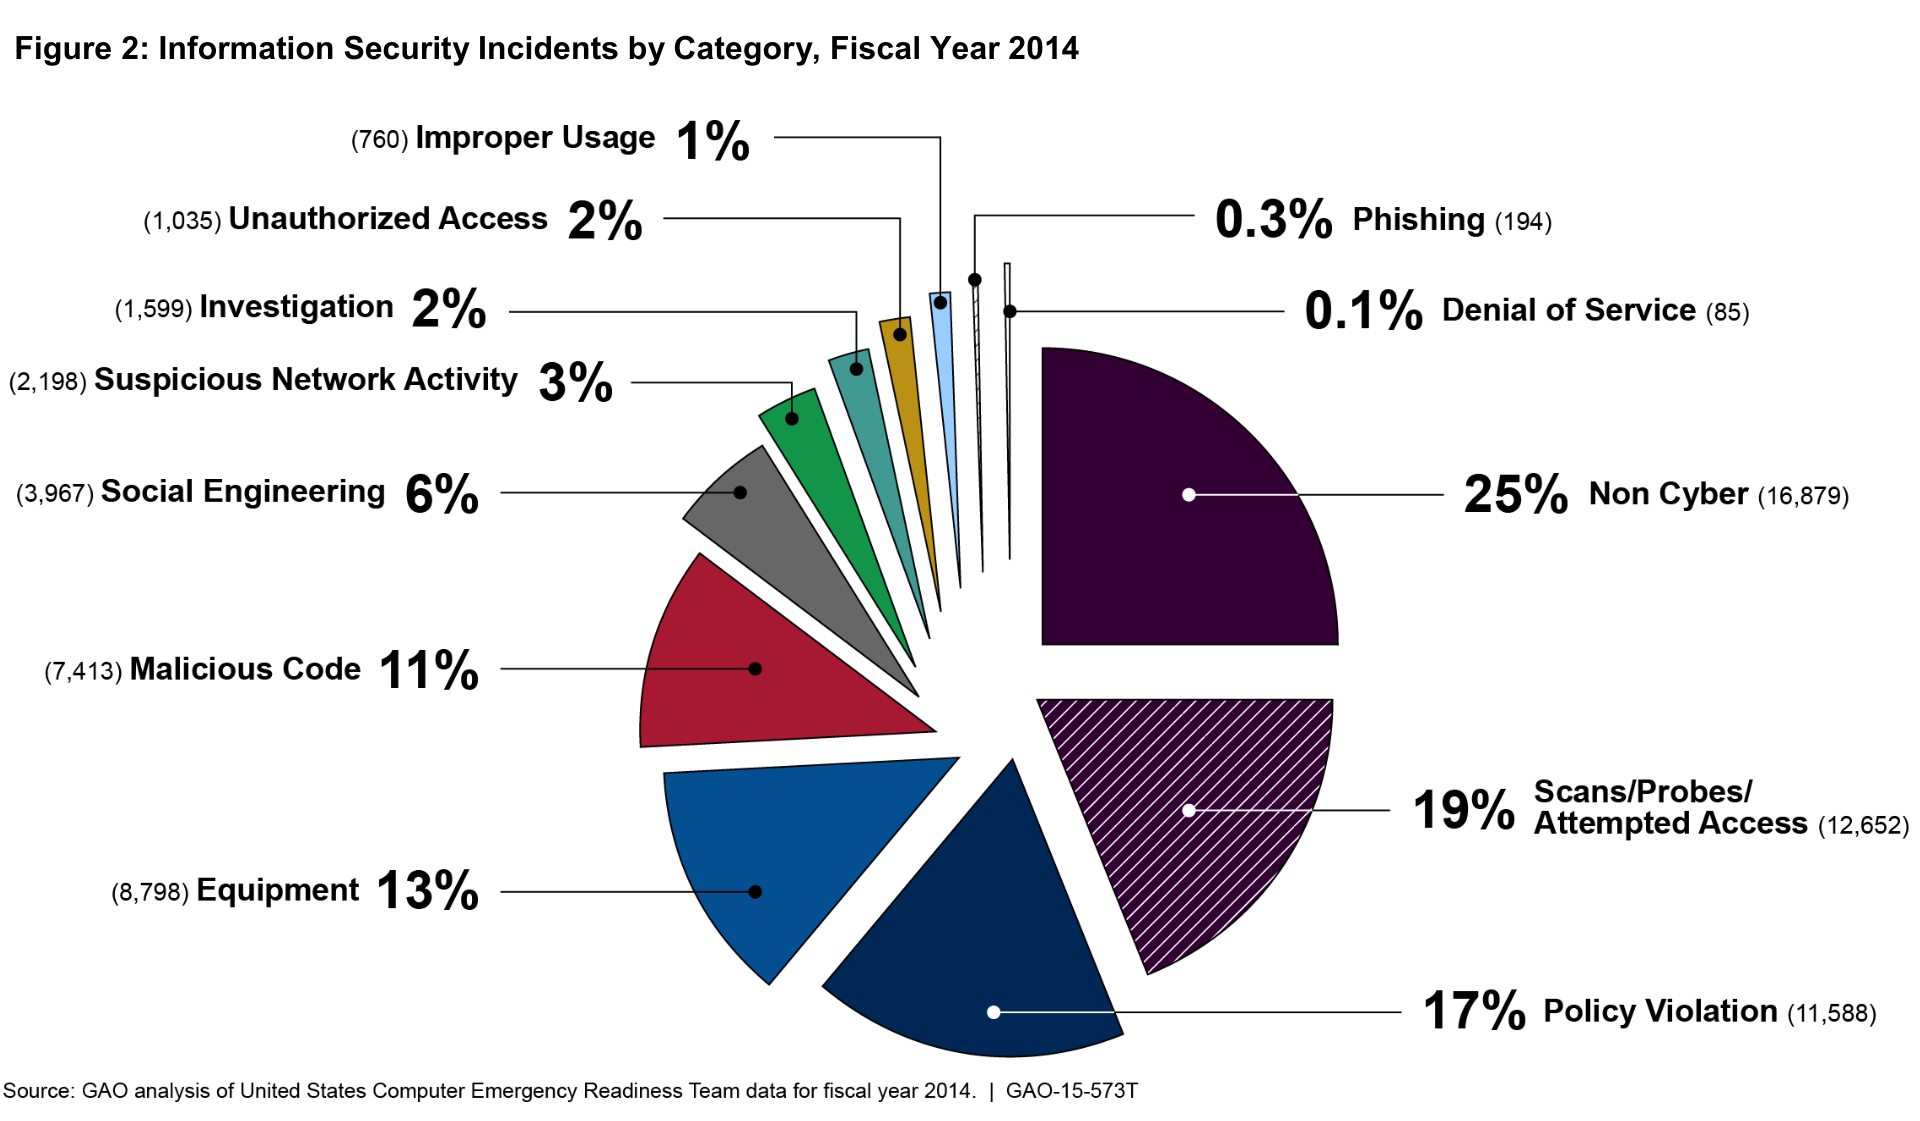
\includegraphics[width=5.511811024in,height=3.65918in]{media/image1.png}

Een grafiek uit het onderzoek van
\textbackslash \cite{Wilshusen2015-rm}. Deze weergeeft dat een groot
deel (74\% uit ongeveer 67.000 meldingen) van alle meldingen van
cybermisdrijven tegenover politici geen meldingen zijn van
cybermisdrijven, maar van pogingen ervan. Dit weergeeft dat er veel
pogingen zijn tot cybermisdrijven, maar dit grotendeels van de tijd niet
lukt of de cybercrimineel geen motivatie meer heeft (hij/zij realiseert
dat het teveel tijd kost, onethisch/moreel is, etc.). Slechts 26\% van
de 67.000 beveiligingsmeldingen zijn niet-cyber-gerelateerd. Het GAO
definieert niet-cyber-gerelateerd als (vrij vertaald): ``\emph{...een
melding van het lekken van PII {[}persoonlijk identificeerbare
informatie{]} of mogelijk verkeerd gebruik van PII waarbij het gaat om
papieren of gedrukt materiaal in tegenstelling tot digitale dossiers.''}

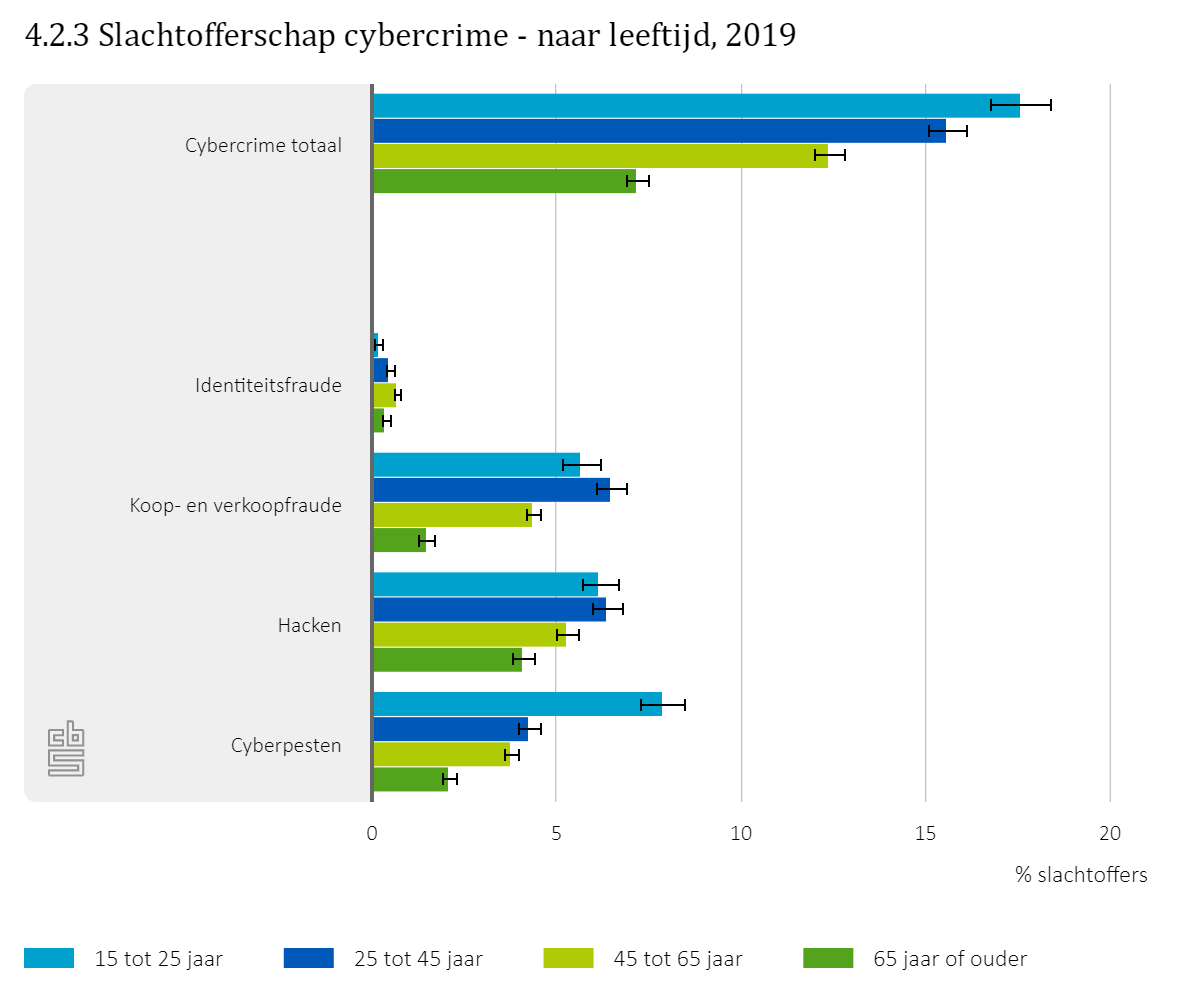
\includegraphics[width=5.511811024in,height=3.67133in]{media/image2.png}

Data van slachtofferschap cybercrime naar leeftijd \cite{CBS2019-ab}. Dit
figuur laat zien dat de Amerikaanse politici qua verhouding van fraude,
hacken en gebruikersfouten in dezelfde lijnen zit als alle meldingen van
cyber misdrijven in de Nederlandse bevolking in 2019 (deze cijfers
zullen niet overeenkomen met die van 2020 of later gezien digitale
identiteitsfraude met meer dan 30\% is gestegen sindsdien, uit onderzoek
van Ministerie van Justitie en Veiligheid, 2021).

Hierbij zijn de wel-cyber-gerelateerde meldingen van:

\begin{enumerate}
\def\labelenumi{\arabic{enumi}.}
\item
  \begin{quote}
  (Dedicated) Denial of Service\\
  Laatst was er een ware epidemie van (D)DoS aanvallen in Nederland
  aanwezig, van Magister, tot bank-apps tot school Wi-Fi. In principe
  betekent dit het overbelasten van een server, een server kan maar een
  bepaald aantal gebruikers aan, als het aantal gebruikers daar boven
  zit, crasht de server.
  \end{quote}
\item
  \begin{quote}
  Hacken\\
  Verreweg de meest bekende vorm van een cyber misdrijf is het hacken
  van een computersysteem. Dit ook, kent veel vormen, bijvoorbeeld het
  bewuste blootleggen of gebruikmaken van een datalek.
  \end{quote}
\item
  \begin{quote}
  Computervirus/-worm\\
  Een computervirus of computerworm is een programma op een computer dat
  zich verspreidt, hierin is ook het verschil tussen een worm en een
  virus zichtbaar. Een virus richt naast het verspreiden van zichzelf
  ook schade aan aan de computer.
  \end{quote}
\item
  \begin{quote}
  Digitale identiteitsfraude\\
  Analoge identiteitsfraude is bij vrijwel iedereen bekend, er is hier
  ook een digitale versie van. Vooral tijdens de COVID-19 pandemie was
  dit steeds populairder aan het worden, er was namelijk op veel plekken
  de mogelijkheid om online een toeslag of uitkering te vragen. Hiervoor
  was het nodig om de identiteit in te voeren. Veel scammers en hackers
  hebben manieren om hier omheen te komen.
  \end{quote}
\item
  \begin{quote}
  Phishing\\
  Het is een steeds bekendere vorm van cyber misdrijf aan het worden; de
  phishing-aanval. Hier maakt iemand een webpagina van een officieel
  bedrijf of overheidsinstelling na. Doordat mensen geen verschillen in
  de echte en nagemaakte website (kunnen) zien, vertrouwen ze de site
  genoeg om persoonlijke informatie erin te voeren. Als aanleiding kan
  de crimineel hierachter identiteitsfraude plegen of ervoor zorgen dat
  mensen vrijwillig geld overmaken bijvoorbeeld.
  \end{quote}
\item
  \begin{quote}
  DNS hijacking\\
  Dit is een dure term die betekent dat als je een webpagina bezoekt,
  een crimineel ervoor kan zorgen dat je een andere website ziet met
  hetzelfde webadres (URL). Dit gaat vaak gepaard met een
  phishing-aanval, maar dat hoeft niet. Er was bijvoorbeeld in 2019 een
  aanval waardoor alle mails van gemeente-officieren voor United Arab
  Emirates werden gestuurd naar criminelen in plaats van de
  gemeente-officieren die ze meenden te e-mailen. De aanval zorgde
  ervoor dat meer dan 50 bedrijven en gemeente-agentschappen mails
  hadden die door werden gestuurd aan de criminelen achter de aanval.
  \end{quote}
\end{enumerate}

Welke redenen zijn er om een cyber misdrijf te plegen?

\begin{enumerate}
\def\labelenumi{\arabic{enumi}.}
\item
  \begin{quote}
  Geld\\
  Cybercriminelen kunnen - meestal door middel van cyberafpersing, het
  gebruik van een virus of de patch van een hack - goed geld verdienen,
  als deze persoon de overweging tussen de beloning en het risico hem of
  haar goede kans vindt geven, zal deze snel het pad van
  cybercriminaliteit volgen.
  \end{quote}
\item
  \begin{quote}
  Macht\\
  Door middel van cyberafpersing kan een cybercrimineel aan veel macht
  komen. Als deze bijvoorbeeld persoonlijke of beveiligde afbeeldingen,
  documenten, etc. op een computer te pakken krijgen en dreigt die
  publiek te maken, belangrijke documenten dreigt te encoderen, of iets
  anders, kan deze politici als poppen voor hem of haar laten dansen.
  \end{quote}
\item
  \begin{quote}
  Publiciteit\\
  Een cybercrimineel kan ook een cyber misdrijf plegen met als doel
  publiciteit te krijgen. Een goed cyberlek dat op professionele manier
  is afgehandeld kan een goede manier zijn om een carrière op te
  starten. Cybercriminelen vergeten vaak dat om dit plan goed te laten
  werken, er eerst toestemming nodig is van de eigenaar. Als dit niet
  het geval is, kunnen ze worden aangeklaagd of geconfronteerd worden
  met een strafrechtelijke rechtszaak.
  \end{quote}
\item
  \begin{quote}
  Wraak\\
  Een bekend motief op veel misdrijven is wraak volgens het onderzoek J.
  Kivivuori et al., 2015, dit is ook zo voor cyber misdrijven. Als
  iemand technisch gericht is en genoeg geduld en vaardigheden heeft,
  kan iemand, uit wraak, uitzoeken hoe je een computer kan hacken of een
  virus kan maken.
  \end{quote}
\item
  \begin{quote}
  Uitdaging\\
  Sommige mensen vinden programmeren te makkelijk of vinden ze het niet
  leuk meer, en zoeken ze meer uitdaging. In plaats van iets
  programmeren, zoeken ze manieren om dingen stuk te maken in plaats van
  te maken.
  \end{quote}
\end{enumerate}

Deze oorzaken zijn de sleutelconcepten van een onderzoek van
\textbackslash \cite{Bell2004-pm}, 2004.
\pagebreak
\hypertarget{criminele-theorieuxebn}{%
\section{Criminele theorieën}\label{criminele-theorieuxebn}}

De meest relevante criminele theorie is die van bioloog Edward Wilson,
sociobiologie. Hij vindt namelijk dat de opvoeding en cultuur niet de
enige factoren zijn die meespelen aan het criminele gedrag. Hij vindt
dat de genetica er ook een grote rol speelt. Agressieve criminelen
hebben bijvoorbeeld vaak een verhoogd testosteronniveau, arrogante
kinderen hebben vaak een lager hartslag, etc. Dit is sinds de ontdekking
van DNA ook geen theorie meer; er is een gen gevonden dat ervoor zorgt
dat de eigenaar eerder crimineel gedrag vertoont. Dit is relevant om de
reden dat leergierigheid en de eigenschap om abstracte onderwerpen
makkelijk te kunnen leren en toepassen genetisch zijn vastgelegd. Mensen
die deze eigenschappen niet hebben, kunnen lastig of helemaal geen cyber
misdrijven plegen.

Daarbij is het aangeleerd gedrag theorie van socioloog Edwin Sutherland
relevant, deze vertelt dat gedrag ook voor een gedeelte bepaald wordt
door de omgeving. Het zegt dat het gezin, de buurt en de vriendengroep
bepalend zijn in het gedrag van de persoon. Als de persoon bijvoorbeeld
bevriend is met criminelen, is de kans een stuk groter dat zij zelf ook
crimineel gedrag vertonen. Deze theorie verklaart bijvoorbeeld ook
software piracy, mensen die leeftijdsgenoten hebben die participeren aan
software piracy, leren en als gevolg ook comfortabeler voelen om het
misdrijf opnieuw te plegen (\textbackslash \cite{Burruss2013-uw},
\textbackslash \cite{Hay2020-an}). Naast software piracy, verklaart
onderdelen van aangeleerd gedrag theorie ook bepaalde cyber misdrijven:
Het leren van programmeren, de normen en waarden om te willen
participeren eraan en het gedrag worden vaak allemaal geleerd van de
omgeving. Het feit dat cybercriminelen ook erg digitaal ondersteund
zijn, betekent ook dat deze mensen online met andere cybercriminelen
kunnen chatten, waar vanwege dezelfde theorie het gedrag wordt
overgenomen.

Daarbij stateert Burrus et al. ook dat zelfcontrole theorie een rol kan
spelen bij software piracy (dit wordt geconfirmeerd door
\textbackslash \cite{Rogers2001-jw} en
\textbackslash \cite{Higgins2004-jy}). Iemand is bijvoorbeeld een stuk
waarschijnlijker om iets illegaal te downloaden als ze impulsief zijn en
dus niet kunnen wachten tot ze het kunnen kopen, daarbij is zo iemand
minder empathisch tegenover de entiteit die de rechten toegeëigend heeft
en negeren ze vaak enige verantwoordelijkheid van het misdrijf. Dit laat
zien dat een persoon met weinig zelfcontrole ook vatbaarder is om cyber
misdrijven te plegen.

Anomietheorie is de theorie die zegt dat criminelen misdrijven plegen
als ze een einddoel hebben dat onbereikbaar is (door discriminatie, geen
diploma, etc.), ``normale'' mensen zullen hun doelen aanpassen,
toekomstige criminelen zullen hierbij misdrijven plegen om toch tot hun
einddoelen te komen. Dit kan bijvoorbeeld het geval zijn met mensen die
professioneel willen programmeren, als ze niet aan een baan komen omdat
hun vaardigheden te laag zijn, proberen ze in een programma in te breken
om te laten zien dat dat niet het geval is.

Rationele keuzetheorie denkt dat criminele afstammen van keuzes, als een
misdrijf plegen de meest gunstige optie is, kiezen criminelen hiervoor
(de pakkans is klein en anders moet je meer werken, dus is stelen de
meest gunstige optie). Dit is een minder relevante theorie, gezien een
cyber misdrijf vaak een grotere pakkans heeft dan andere misdrijven en
het vrijwel altijd minder opbrengsten geeft.

De bindingstheorie vindt dat ieder mens een crimineel in zich hebben
schuilen, maar dat de mogelijkheid om alles op het spel te zetten een
crimineel maakt is ook iets minder relevant, er zijn veel mensen die
niet technisch of intellectueel genoeg gesteld zijn om een cyber
misdrijf te plegen, deze theorie is logisch voor criminaliteit in het
algemeen, maar niet voor specifiek cybercrime.

Psychoanalyse is de theorie van Sigmund Freud die zegt dat een
balansverstoring tussen instinctieve driften, het ego en het superego
crimineel gedrag veroorzaakt. Deze is minder relevant, gezien er geen
bewijs is gevonden dat er een balansverstoring is tussen de behoefte aan
onmiddellijke voldoening van fysieke behoeften, gebrek of overschot aan
rationele redenering en gebrek of overschot sociale regels of morelen
bij mensen die cyber misdrijven plegen.
\pagebreak
\hypertarget{welke-wetten-zijn-er-tegen-cybercriminelen}{%
\section{\texorpdfstring{Welke wetten zijn er \emph{tegen}
cybercriminelen?}{Welke wetten zijn er tegen cybercriminelen?}}\label{welke-wetten-zijn-er-tegen-cybercriminelen}}

\hypertarget{cyber-aanvallen-op-informatiesystemen}{%
\subsection{Cyber aanvallen op
informatiesystemen}\label{cyber-aanvallen-op-informatiesystemen}}

(\href{https://wetten.overheid.nl/jci1.3:c:BWBR0001854\&boek=Tweede\&titeldeel=V\&artikel=138ab\&z=2021-07-01\&g=2021-07-01}{\underline{art.
138ab}})

Volgens artikel 138ab is het strafbaar om in te breken in een beveiligd
systeem, data af te tappen, brute-force-aanvallen te plegen of een
botnet te maken. Dit houdt in dat vrijwel alle acties om beveiliging
digitaal te omzeilen illegaal is. In wetsartikel 138ab wordt niet
genoemd dat dit legaal wordt na toestemming, dus zelfs als je een
contract afsluit met het bedrijf voor het opzoeken van bugs binnen de
beveiliging, kan je vervolgd worden.

\hypertarget{gebruik-van-botnets}{%
\subsection{Gebruik van botnets}\label{gebruik-van-botnets}}

(\href{https://wetten.overheid.nl/jci1.3:c:BWBR0001854\&boek=Tweede\&titeldeel=V\&artikel=139d\&z=2021-07-01\&g=2021-07-01}{\underline{art.
139d}})\\
Volgens wetsartikel 139d, is het illegaal om een botnet te maken, met
welk doel dan ook. Een botnet is een soort worm, een programma dat zich
tussen meerdere computers verspreid met een specifiek doel.

Wel opvallend is dat
\href{https://www.rijksoverheid.nl/onderwerpen/cybercrime-en-cybersecurity/cybercriminaliteit-bestrijden}{\underline{een
webpagina van de officiële rijksoverheid pagina}} noemt ``Met botnets
nemen criminelen bijvoorbeeld computers over. Op die manier krijgen ze
toegang tot privégegevens.''. Dit is gemiddeld genomen niet het doel van
een botnet. Neem het malware van de WannaCry-aanval in 2017 als
voorbeeld, deze maakte gebruik van een botnet om zichzelf te
verspreiden. Een botnet wordt grotendeels van de tijd gebruikt om de
volgende redenen:

\begin{enumerate}
\def\labelenumi{\arabic{enumi})}
\item
  \begin{quote}
  Cyberafpersing, het verspreidt zich en versleutelt privédocumenten
  (zoals te zien in de WannaCry-aanval van 2017)
  \end{quote}
\item
  \begin{quote}
  Het overbelasten van netwerken, door veel computers meerdere pakketten
  naar een bepaalde pagina te sturen, kan het deze platleggen (zoals te
  zien met het Mirai-botnet).
  \end{quote}
\item
  \begin{quote}
  Het verhogen van verwerkingscapaciteit door een netwerk aan te leggen,
  bijvoorbeeld om grootschalig bitcoin te minen (zoals te zien met het
  Sysrv-botnet)
  \end{quote}
\end{enumerate}
\pagebreak
\hypertarget{welke-rechten-hebben-cybercriminelen}{%
\section{Welke rechten hebben
cybercriminelen?}\label{welke-rechten-hebben-cybercriminelen}}

Als iemand per ongeluk een cyber misdrijf pleegt, bijvoorbeeld door per
ongeluk iets uit te proberen zonder eerst toestemming te vragen om het
systeem te penetreren, zijn er ook rechten om deze mensen te beschermen.
Op deze manier zijn jongeren die leren hoe cybercrime werkt, vrijwel
volledig beschermt, zolang het per ongeluk aangerichte
computervredebreuk is. Deze zijn vooral opgericht met het doel om
jongeren verder te onderwijzen in de cyber-sector, zodat ze meer
richting het beveiligen van systemen werken dan de richting van cyber
misdrijven plegen. Hier zijn een paar voorbeelden van rechten:

\hypertarget{computervredebreuk}{%
\subsection{Computervredebreuk}\label{computervredebreuk}}

(\href{https://wetten.overheid.nl/jci1.3:c:BWBR0001854\&boek=Tweede\&titeldeel=V\&artikel=138ab\&z=2021-07-01\&g=2021-07-01}{\underline{art.
138ab}})

Art. 138ab van het Wetboek van Strafrecht impliceert dat het alleen
strafbaar is als de computervredebreuk gepland en opzettelijk was; ``hij
die opzettelijk en wederrechtelijk binnendringt''. Dit heeft hetzelfde
probleem als het wetsartikel voor moord, als er geen opzet in het spel
was en er geen voorbedachte rede te bewijzen valt, is dit niet te
veroordelen. Daarbij is ethisch hacken, of hacken om een dienst voor het
bedrijf te betekenen, ook niet hiermee inbegrepen, zolang het van
tevoren gemeld wordt bij het desbetreffend bedrijf.

\hypertarget{hack_right}{%
\subsection{Hack\_Right}\label{hack_right}}

(sinds 2018 in proefperiode,
\href{https://www.dehaagsehogeschool.nl/docs/default-source/documenten-onderzoek/lectoraten/cybersecurity-in-het-mkb/hack_right.pdf}{\underline{Schiks,
J. A. M., Van 't Hoff-de Goede, M. S., \newline \& Leukfeldt, E. R. (2018).}
\emph{\underline{Een alternatief voor jeugdige hackers?}}
\newline
\underline{Nederlands Studiecentrum Criminaliteit en
Rechtshandhaving.}})

Dit recht is vooral belangrijk te benoemen wegens het doel van dit
artikel, leerlingen van de Haagse Hogeschool waren van mening dat het
straffen van minderjarigen een beter doel zou moeten hebben dan
straffen. Het moest gericht worden op de heropvoeding van minderjarige
hackers. Dit recht houdt in dat jongeren niet naar de jeugdgevangenis
worden gestuurd na het plegen van een cyber misdrijf, maar juist worden
opgeleid in het ethisch hacken, een stage krijgen aangeboden en een plek
te vinden waar ze zich veilig voelen. Hiermee kunnen ze meer leren over
het beveiligen van een systeem zodat hier niet binnen te dringen valt,
in plaats van het leren van hoe je op een plek kan binnendringen.

\hypertarget{meldplicht-wbp}{%
\subsection{Meldplicht Wbp}\label{meldplicht-wbp}}

(\href{https://wetten.overheid.nl/jci1.3:c:BWBR0011468\&hoofdstuk=2\&paragraaf=1\&artikel=13\&z=2018-05-01\&g=2018-05-01}{\underline{art.
13 Wbp}} \&
\href{https://wetten.overheid.nl/BWBR0037346/2015-12-16}{\underline{Meldplicht
datalekken Wbp}})

De Meldplicht datalekken en artikel 13 van Wet bescherming
persoonsgegevens zeggen dat als je een datalek vindt, je deze verplicht
bent te melden. Dit houdt in dat als je probeert iets te hacken, voordat
je een melding maakt met de reden pas de medewerkers te storen als het
niet genoeg beveiligd is, je wel gelijk verplicht bent het te melden als
je iets hebt gevonden. Als je dit na het ontdekken van het lek pas doet,
ben je strafbaar.

\hypertarget{wet-computercriminaliteit-iii-art.-139g}{%
\subsection{\texorpdfstring{Wet Computercriminaliteit III\\
(\href{https://wetten.overheid.nl/jci1.3:c:BWBR0001854\&boek=Tweede\&titeldeel=V\&artikel=139g\&z=2021-07-01\&g=2021-07-01}{\underline{art.
139g}})}{Wet Computercriminaliteit III (art. 139g)}}\label{wet-computercriminaliteit-iii-art.-139g}}

Volgens wetsartikel 139g lid 2, Computercriminaliteit III, is niet
strafbaar degene die te goeder trouw heeft kunnen aannemen dat het
algemeen belang het verwerven, voorhanden hebben, ter beschikking
stellen, bekendmaken of gebruik van de gegevens, bedoeld in het eerste
lid, vereiste. Dit houdt in dat iemand die met goede bedoelingen een lek
vindt en daarna ook direct meldt zonder de gevonden lek of data die het
oplevert aan een ander doorgeeft of publiceert vrijwel immuun is tegen
aanklacht of dergelijke.
\pagebreak
\hypertarget{doelen-van-de-straffen}{%
\section{Doelen van de straffen}\label{doelen-van-de-straffen}}

\hypertarget{vergelding}{%
\subsection{Vergelding}\label{vergelding}}

Vergelding, beter bekend als wraak, is het iemand laten voelen wat hij
heeft gedaan. Wie een strafbaar feit heeft begaan, mag daar niet mee
wegkomen. Hij verdient straf. Het slachtoffer en de samenleving
verdienen genoegdoening. Dit is relevant voor cyber misdrijven omdat er
een gevangenisstraf op staat, het slachtoffer van de cyberaanval krijgt
genoegdoening van de straf. De gevangenisstraf op cyber misdrijven is
maximaal 5 jaar, dat betekent dat er naast vergelding een ander, meer
relevant doel aanwezig is.

\hypertarget{preventie}{%
\subsection{Preventie}\label{preventie}}

Preventie moet ervoor zorgen dat de dader het misdrijf niet opnieuw wil
plegen. Ook zorgt preventie ervoor dat anderen niet de fout in gaan als
ze zien dat het daadwerkelijk een strafbaar feit is. Preventie is een
minder relevant doel, gezien de overheid er niet voor wil zorgen dat de
misdadiger niet meer datalekken vindt en gebruikt, ze wilt ervoor zorgen
dat de misdadiger het niet meer \emph{illegaal} doet. Er is een groot
tekort aan professionele bug bounties en ICT'ers over het algemeen, het
demotiveren van die sector met straffen zorgt ervoor dat er nog een
groter tekort komt.

\hypertarget{beveiliging-van-de-maatschappij-en-burgers}{%
\subsection{Beveiliging van de maatschappij en
burgers}\label{beveiliging-van-de-maatschappij-en-burgers}}

De dader die een misdrijf pleegt zit voor een bepaalde tijd, kan voor
die tijd geen misdrijven meer plegen. De samenleving is dan (tijdelijk)
beschermd tegen deze persoon. Deze is voor dezelfde reden als vergelding
iets minder relevant, de gevangenisstraffen en boetes zijn te laag om
beveiliging van de maatschappij en burgers als doel te hebben.

\hypertarget{handhaving-van-de-rechtsorde-en-het-voorkomen-van-eigenrichting}{%
\subsection{Handhaving van de rechtsorde en het voorkomen van
eigenrichting}\label{handhaving-van-de-rechtsorde-en-het-voorkomen-van-eigenrichting}}

Een straf kan ervoor zorgen dat iemand die probeert voor eigen rechter
te spelen dat niet meer kan doen, zodat de rechtsorde weer aan gang kan
en echte rechters voor rechter spelen. Deze kan relevant zijn, maar dat
ligt aan het geval. Als een cyber-misdadiger voor eigen rechter speelt
en andere misdadigers hackt, kan dit een relevant doel zijn. Anders
niet.

\hypertarget{resocialisatie}{%
\subsection{Resocialisatie}\label{resocialisatie}}

Sommige straffen, zoals Hack\_Right, zijn meer gericht op de
heropvoeding van de misdadiger. Deze zorgen ervoor dat de misdadiger
leert wat goed en slecht is, leert wat hij/zij heeft beschadigt en
misschien ook leert om te helpen het goede te doen. In het voorbeeld van
Hack\_Right, zorgt dat voor al deze dingen. Jonge hackers worden in
plaats van gestraft, opgenomen in het ICT van de overheid en worden
allerlei dingen geleerd. Dan krijgen ze ook geen strafblad, met de
waarschuwing dat dat wel gebeurt als ze het nog een keer proberen. Deze
is dus relevant, voor dezelfde reden dat preventie irrelevant is, het
zorgt ervoor dat cyber-misdadigers hun intellect en kennis voor goede
doelen gebruiken, zoals programmeren of bug bounty doeleinden. Het zorgt
ervoor dat in plaats van het verminderen van het aantal ICT'ers in
Nederland, het aantal ICT'ers hetzelfde blijft of zelfs groeit.

\hypertarget{genoegdoening}{%
\subsection{Genoegdoening}\label{genoegdoening}}

Een straf zorgt ervoor dat het gezin van de slachtoffer en/of
slachtoffer zelf genoegdoening krijgt, dat ze weer emotioneel en fysiek
kunnen herstellen. Dit is ook relevant, omdat het slachtoffer van een
cyber-misdrijf vaak een bedrijf is, deze heeft tijd nodig om te
herstellen.

Deze strafdoelen komen uit een onderzoek van \emph{1.5
\textbackslash \cite{Gardiner1958-we}} en worden gebruikt in Arizona
strafrecht, zie \emph{2005 Arizona Revised Statutes - :: Revised
Statutes §13-901.01 Probation for Persons Convicted of Possession or Use
of Controlled Substances or Drug Paraphernalia; Treatment; Prevention;
Education; Definition}, z.d.
\pagebreak
\hypertarget{conclusie}{%
\section{Conclusie}\label{conclusie}}

Uit het onderzoek is gebleken dat alle soorten cybercrime illegaal zijn
met de uitzondering van cybercrime met toestemming van het slachtoffer
zogezegd. Dit contract kan mondeling, informeel via e-mail of anders
zijn, zolang er dossier van is. Straffen tegen cybercriminelen hebben
maximaal 5 jaar celstraf of geldboete van de vierde graad (maximaal
€21.750) met -- gemiddeld gesproken -- als doel resocialisatie,
genoegdoening of het voorkomen van eigenrichting.

Cybercriminelen zijn vaak aangeboren en product van hun directe
omgeving, aldus de relevante criminele theorieën van Edward Wilson,
Edwin Sutherland en Robert Merton. In de praktijk is dat ook te zien,
cybercriminelen komen vaak van rijkere buurten, hebben in veel gevallen
een hoger IQ dan het landelijk gemiddelde en hebben vaak mensen in hun
directe omgeving veel te doen met technologische ontwikkelingen, worden
zelf opgevoed met technologische ontwikkelingen zoals huiswerk moeten
maken in een digitale omgeving of een combinatie van de bovenstaande.

Er zijn 6 voornamelijke vormen van cybercrime, die ongeveer ¼ van alle
meldingen van Amerikaanse politici opmaken, de andere ¾ zijn
gebruikersfouten (exclusief aanvallen op het vertrouwen van de politici
buiten scams, bijvoorbeeld phishing-aanvallen) of hebben niet datalekken
of andere ICT-gerelateerde problemen als oorzaak (zoals cyberpesten),
die één of meer van 5 doelen op het oog hebben.
\pagebreak
\hypertarget{conflict-of-interest}{%
\section{Conflict of Interest}\label{conflict-of-interest}}

De schrijver van dit onderzoek, Luc Angevare, is een programmeur en
(ethisch) hacker. Hij heeft in 4 verscheidene websites die de school
gebruikte datalekken gevonden en gemeld. Samen met het feit dat hij
server-side websites programmeert, is hij van mening dat het mogelijk
moet zijn om eerst een datalek te zoeken, en pas te melden zodra er iets
gevonden is. Op deze manier is alles veiliger te maken zonder het risico
dat men gevaar loopt aangeklaagd te worden. Pas als er bewust schade is
aangericht na het vinden van de lek, moet het mogelijk zijn om de dader
aan te klagen.

De wet in zijn huidige staat zegt dat er eerst om toestemming gevraagd
moet worden voordat een speurtocht naar potentiële datalekken mag
plaatsvinden. Als programmeur, scholier, iemand die geeft om zijn
privacy en het vertrouwen dat hij confidentiële informatie kan invoeren
zonder dat een derde, ongeautoriseerde persoon dat kan lezen vindt Luc
dat abnormaal. Men mag rondvragen om te testen of een dokter of
psycholoog zich aan de beroepsgeheim houdt, maar testen om te kijken of
een website veilig is en of de spreekwoordelijke data tunnel geen lekken
bevat mag niet zonder toestemming.

Een van de websites die wij moesten gebruiken waar hij een lek in vond,
was een website waar je stellingen in moest voeren waaraan je probeert
te verbeteren en daarvoor ervaringen in moet voeren. Het was voor hem
belangrijk om te testen of deze door een derde hieraan mee kon lezen,
iemand die van alle leerlingen op deze school geautomatiseerd deze
ervaringen kan bekijken, kan in sommige gevallen zelfs te weten komen
waar deze woont.

Tegelijkertijd zal een groot uitgeversbedrijf als Noordhoff nooit
toestemming verlenen aan een leerling uit leerjaar 3 om bewust te
proberen een website te hacken met het vermoeden (en niets anders) dat
deze het lek, als ze deze vinden, aan het bedrijf melden en aan niemand
anders vertelt of publiceert. Naar Luc's ervaring, zijn juist deze
bedrijven degenen die het minst uitgeven aan beveiliging, maar juist wel
genoeg uit kunnen geven aan een rechtszaak in het privaatrecht.

Een groot deel van de strafrechtelijke wetsartikelen zijn geschreven
vanuit het perspectief van bescherming van grote bedrijven en de
technische ontwikkelingen ervan, in plaats van het perspectief van de
gebruikers, die er zeker van moeten zijn dat hun gegevens beschermd
blijven en niet openbaar gemaakt kunnen worden, legaal of illegaal.

In de informatiemaatschappij waar wij nu leven, moet het mogelijk zijn
om te testen of een website waar je vertrouwelijke informatie in moet
voeren wel veilig is en er geen data afgetapt kan worden. Volgens het
WBP moet een bedrijf een poging doen om hun website zo veilig mogelijk
te maken zodat persoonlijke informatie niet makkelijk gestolen kan
worden, maar naar Luc's ervaring gebeurt dit lang niet altijd. Iemand
kan er nooit achter komen of het bedrijf zich aan deze plicht houdt
tenzij ze de wet breken of zich voordoen als bug bounty.

\textbf{Als scholier lijkt het mij niet fijn om een nieuwe FaceMash te
krijgen met mijn gezicht erop.}

\hypertarget{referenties}{%
\bibliography{referenties}}

\end{document}
